\documentclass[]{article}

\usepackage{amsmath}
\usepackage{graphicx}
\usepackage{amssymb}
\usepackage{esdiff}
\usepackage{hyperref}
\graphicspath{.}

%opening
\title{Double Pendulum: Theory}
\author{Ben Hoberman}

\begin{document}
	
\date{June 17, 2017 -- July 25, 2017}
\maketitle

\newcommand{\lagr}{\mathcal{L}}

\section{Introduction}
After finishing my first year of mechanics, I figured that simulating something a little more complicated than what we studied in class might be interesting. I encountered the problem of the double pendulum and decided I'd try my hand at it. Some research divulged that Lagrangian mechanics could give me an easier way to understand the behavior of the system, so after some research and an MIT online lecture (available \href{https://www.youtube.com/watch?v=zhk9xLjrmi4&t=3925s}{here}), this is my attempt at figuring out a double pendulum.

\section{Notes}
To make some of this math more readable, I'll be omitting the dependence of $\theta$'s and their derivatives on $t$ and other variables. Instead of $\theta{(t)}$, you'll just see $\theta$. Also to reduce clutter, I'll be using dot notation to indicate time derivatives, so $\dot{\theta}$ means $\diff{\theta}{t}$. To avoid introducing errors (and to save my sanity), most of the symbolic math was done in sympy. The code I wrote for those symbolic calculations can be found in the symmath.py file in this repository.

\section{Describing the System}
\begin{figure}[h!]
	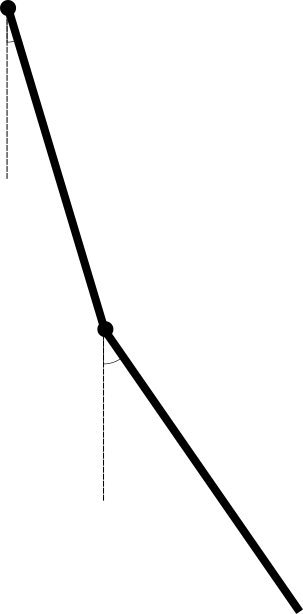
\includegraphics[height=5cm]{situation}
	\caption{A crude image of a double pendulum}
\end{figure}
$\theta_1$ represents angle between the anchored stick and the vertical, and $\theta_2$ represents the the angle between the free stick and the vertical. Both increase with counterclockwise rotation. The anchored stick has length $l_1$ and mass $m_1$, while the free stick has length $l_2$ and mass $m_2$.

In order to write the Lagrangian for this system, we need to choose a generalized coordinate system and express the system's kinetic and potential energies in terms of those coordinates. We will use $\theta_1$ and $\theta_2$ as our system's independent generalized coordinates.

The two sticks are the only elements of the system that account for its kinetic energy. All of the anchored stick's kinetic energy can be easily expressed as rotational kinetic energy, but the free stick will have a translational kinetic energy in addition to a rotational one, both calculated most easily about the stick's center.

In order to calculate the translational speed of the center of mass of the free stick, we have do some math. The cartesian coordinates of the centers of mass of the two sticks are as follows:
\begin{gather*}
x_1 = \frac{l_1}{2}\sin(\theta_1) \\
y_1 = -\frac{l_1}{2}\cos(\theta_1) \\
x_2 = l_1\sin(\theta_1) + \frac{l_2}{2}\sin(\theta_2) \\
y_2 = -l_1\cos(\theta_1) - \frac{l_2}{2}\cos(\theta_2)
\end{gather*}
In order to find the linear velocity, we can use the good old Pythagorean theorem to figure out that $v = \sqrt{\dot{x}^2 + \dot{y}^2}$, or, even more conveniently, that $v^2 = \dot{x}^2 + \dot{y}^2$ for the free stick stick. Let's do that:
\begin{gather*}
	v_2^2 = \dot{x_2}^2 + \dot{y_2}^2 = (\dot{\theta_1}l_1\cos(\theta_1) + \dot{\theta_2}\frac{l_2}{2}\cos(\theta_2))^2 + (\dot{\theta_1}l_1\sin(\theta_1) + \dot{\theta_2}\frac{l_2}{2}\sin(\theta_2))^2 \\
	= \dot{\theta_1}^2l_1^2 + \frac{\dot{\theta_2}^2l_2^2}{4} + \dot{\theta_1}\dot{\theta_2}l_1l_2\cos(\theta_1 - \theta_2) \\
	K_{\text{linear}} = \frac12m_2v_2^2 = \frac12m_2(\dot{\theta_1}^2l_1^2 + \frac{\dot{\theta_2}^2l_2^2}{4} + \dot{\theta_1}\dot{\theta_2}l_1l_2\cos(\theta_1 - \theta_2)) \\
	= \frac12m_2\dot{\theta_1}^2l_1^2 + \frac18m_2\dot{\theta_2}^2l_2^2 + \frac12m_2\dot{\theta_1}\dot{\theta_2}l_1l_2\cos(\theta_1 - \theta_2)
\end{gather*}
Because our selected independent coordinates describing the system are $\theta_1$ and $\theta_2$, describing the rotational kinetic energy of the system is much more simple. For each stick, $K_{rot} = \frac12 I \dot{\theta}^2$. The anchored stick has moment of intertia $\frac13m_1l_1^2$, and the free stick has moment of intertia $\frac{1}{12}m_2l_2^2$.
\begin{gather*}
	K_{\text{rotational}} = \frac16m_1l_1^2\dot{\theta_1}^2 + \frac{1}{24}m_2l_2^2\dot{\theta_2}^2
\end{gather*}

We can now find the total kinetic energy of the system:
\begin{gather*}
	K = K_{linear} + K_{rot} \\
	= \frac12m_2\dot{\theta_1}^2l_1^2 + \frac18m_2\dot{\theta_2}^2l_2^2 + \frac12m_2\dot{\theta_1}\dot{\theta_2}l_1l_2\cos(\theta_1 - \theta_2) + \frac16m_1l_1^2\dot{\theta_1}^2 + \frac{1}{24}m_2l_2^2\dot{\theta_2}^2
\end{gather*}

In order to find the Lagrangian of the system, we must also describe the potential energy of the system at any given time. Gravitational potential energy accounts for the potential energy in this system, so let's figure out the gravitational potential energy of the system. It doesn't actually matter where we pick the zero position to be, so we'll call the horizontal zero in order to simplify the expression (because $\cos(\frac{\pi}{2}) = 0$, and the horizontal is at $\frac{\pi}{2}$ in our system):
\begin{gather*}
	U_g = \sum mg\Delta h = m_1gy_1 + m_2gy_2 \\
	= -\frac{l_1m_1g}{2}\cos(\theta_1) - m_2g(l_1\cos(\theta_1) + \frac{l_2}{2}\cos(\theta_2)) \\
	= -g\cdot\frac{l_1m_1\cos(\theta_1) + 2m_2l_1\cos(\theta_1) + m_2l_2\cos(\theta_2)}{2} \\
	= -g\cdot\frac{(l_1m_1 + 2m_2l_1)\cos(\theta_1) + m_2l_2\cos(\theta_2)}{2} \\
	= -\frac{g}{2}(l_1m_1 + 2m_2l_1)\cos(\theta_1) - \frac{g}{2}m_2l_2\cos(\theta_2)
\end{gather*}

Now that we have calculated the kinetic and potential energies of the system, we can calculate the Lagrangian, $\lagr = K - V$, where $K$ is the total kinetic energy and $V$ is the total potential energy:
\begin{gather*}
	\lagr = K - V = \frac{1}{2}g l_1  m_1 \cos{ (\theta_1  )} + g l_1 m_2 \cos{ (\theta_1  )} + \frac{1}{2}g l_2  m_2 \cos{ (\theta_2  )} \\ + \frac{1}{6}l_1^2 m_1  \dot{\theta_1}^2 + \frac{1}{2}l_1^2 m_2  \dot{\theta_1}^2 + \frac{1}{2}l_1 l_2  m_2 \cos{ (\theta_1 - \theta_2  )} \dot{\theta_1} \dot{\theta_2} + \frac{1}{6}l_2^2 m_2  \dot{\theta_2}^2
\end{gather*}

With the Lagrangian, we can set up the Euler-Lagrange differential equation for each coordinate:
\begin{gather*}
	\diff{}{t}\frac{\partial \lagr}{\partial \dot{\theta_1}} = \frac{\partial \lagr}{\partial \theta_1} \\ \\
	\diff{}{t}\frac{\partial \lagr}{\partial \dot{\theta_2}} = \frac{\partial \lagr}{\partial \theta_2}
\end{gather*}

We can now solve these two differential equations for $\ddot{\theta_1}$ and $\ddot{\theta_2}$, which together will be used in our simulation. I did this entire process using sage and would not recommend trying it by hand. I have decided not to include any of the equations in the process here because they look gross, but you can check out the sage notebook if you're interested.

\begin{gather*}
	N_1 = l_1 m_2 {\dot{\theta_1}}^{2} \cos({\theta_2} - {\theta_1}) \sin({\theta_2} - {\theta_1}) + 2  l_2 m_2 {\dot{\theta_2}}^{2} \sin({\theta_2} - {\theta_1}) \\ + g m_2 \cos({\theta_2} - {\theta_1}) \sin({\theta_2}) - 2  {(g m_1 + 2  g m_2)} \sin({\theta_1}) \\
	\ddot{\theta_1} = -3\frac{N_1}{3  l_1 m_2 \cos({\theta_2} - {\theta_1})^{2} - 4  l_1 m_1 - 12  l_1 m_2} \\
	N_2 = 3  l_2 m_2 {\dot{\theta_2}}^{2} \cos({\theta_2} - {\theta_1}) \sin({\theta_2} - {\theta_1}) - 3  {(g m_1 + 2  g m_2)} \cos({\theta_2} - {\theta_1}) \sin({\theta_1}) \\ + 2  g m_1 \sin({\theta_2}) + 6  g m_2 \sin({\theta_2}) + 2  {(l_1 m_1 {\dot{\theta_1}}^{2} + 3  l_1 m_2 {\dot{\theta_1}}^{2})} \sin({\theta_2} - {\theta_1}) \\
	\ddot{\theta_2} = \frac{N_2}{3  l_2 m_2 \cos({\theta_2} - {\theta_1})^{2} - 4  l_2 m_1 - 12  l_2 m_2}
\end{gather*}

We now have a pair of second order differential equations that describes the motion of the system. Using the Runge-Kutta method (aka RK4), we can approximate solutions for $\theta_1$ and $\theta_2$ over some time interval. First, let us redefine this system as a single vector function:

\begin{gather*}
	\theta = 
	\begin{bmatrix}
		\theta_1 \\
		\theta_2
	\end{bmatrix} \text{, }
	\dot{\theta} = 
	\begin{bmatrix}
		\dot{\theta_1} \\
		\dot{\theta_2}
	\end{bmatrix} \text{, and }
	\ddot{\theta} =
	\begin{bmatrix}
		\ddot{\theta_1} \\
		\ddot{\theta_2}
	\end{bmatrix} \\
	\ddot{\theta}(\theta, \dot{\theta}) = \boldsymbol{A}^{-1}\vec{b}\text{, according to $\boldsymbol{A}(\theta, \dot{\theta})$ and $\vec{b}(\theta, \dot{\theta})$ above}
\end{gather*}

Now we will set up the RK4 method for this system.

\begin{gather*}
	\text{Let } z = \dot{\theta}(\theta, \dot{\theta}) = \diff{\theta}{t} \text{, so } \diff{z}{t} = \ddot{\theta} \\
	z = \dot{\theta} \\
	\dot{z} = \ddot{\theta}(\theta, \dot{\theta}) \\
	\theta_{new} = \theta + \frac{h}{6}(k_0 + 2k_1 + 2k_2 + k_3) \\
	\dot{\theta}_{new} = \dot{\theta} + \frac{h}{6}(l_0 + 2l_1 + 2l_2 + l_3) \\
	\text{Let our step be $h$, and $k$ and $l$ are as follows:}\\
	k_0 = hz = h\dot{\theta}_0 \\
	l_0 = h\dot{z} = h\ddot{\theta}_0 \\
	k_1 = hz(\theta_0 + \frac{k_0}{2}, \dot{\theta}_0 + \frac{l_0}{2}) = h\cdot(\dot{\theta}_0 + \frac{l_0}{2}) \\
	l_1 = h\dot{z}(\theta_0 + \frac{k_0}{2}, \dot{\theta}_0 + \frac{l_0}{2}) = h\cdot\ddot{\theta}(\theta_0 + \frac{k_0}{2}, \dot{\theta}_0 + \frac{l_0}{2}) \\
	k_2 = hz(\theta_0 + \frac{k_1}{2}, \dot{\theta}_0 + \frac{l_1}{2}) = h\cdot(\dot{\theta}_0 + \frac{l_1}{2}) \\
	l_2 = h\dot{z}(\theta_0 + \frac{k_1}{2}, \dot{\theta}_0 + \frac{l_1}{2}) = h\cdot\ddot{\theta}(\theta_0 + \frac{k_1}{2}, \dot{\theta}_0 + \frac{l_1}{2}) \\
	k_3 = hz(\theta_0 + k_2, \dot{\theta}_0 + l_2) = h\cdot(\dot{\theta}_0 + l_2) \\
	l_3 = h\dot{z}(\theta_0 + k_2, \dot{\theta}_0 + l_2) = h\cdot\ddot{\theta}(\theta_0 + k_2, \dot{\theta}_0 + l_2)
\end{gather*}

Implementing this in code will get us our simulation. Hopefully.

\end{document}
